\subsection{Die magnetischen Momente eines Elektrons}

Elektronen, die sich auf bestimmten Hüllen im Atom befinden, können durch die Quantenzahlen ($n, l, m, s$) beschrieben werden.
Dabei beschreiben $l$ und $s$ den Bahndrehimpuls und den Spin (also den Eigendrehimpuls) der Elektronen und $n$ ist
die Hauptquantenzahl. Je nach Hauptquantenzahl können $l$ und $s$ unterschiedliche Werte annehmen. Allgemein gilt für die
Beträge des Drehimpulses bzw. Spins:

\begin{align}
	|\vec{l}| = \hbar \sqrt{l(l+1)}&\text{ mit } l=0,1,\hdots,n-1\\
	|\vec{s}| = \hbar \sqrt{s(s+1)}&\text{ mit } s=\frac{1}{2}
\end{align}

Die beiden magnetischen Momente errechnen sich aus

\begin{align}
	|\vec{\mu}_l| = -\mu_{B} \sqrt{l(l+1)} \\
	|\vec{\mu}_s| = - g_{s} \mu_{B} \sqrt{s(s+1)} ,
\end{align}

wobei $\mu_B$ das Bohrsche Magneton und $g_s \approx 2$ der gyromagnetische Faktor ist.

\subsection{LS- und jj-Kopplung}

Je nach Kernladungszahl $Z$ liegt eine andere Art von Spin-Bahn-Wechselwirkung vor. Bei geringen $Z$ dominiert die LS-Kopplung.
Das bedeutet, dass die Kopplung zwischen dem Spin- und dem Bahndrehimpulsmoment eines Teilchens klein gegenüber der
Kopplung zwischen verschiedenen Hüllenelektronen ist.

Diese koppeln dann nämlich zu einem Gesamtbahndrehimpuls und einem Gesamtspin

\begin{align}
	\vec{L} &= \sum \vec{l}_i\\
	\text { und }\\
	\vec{S} &= \sum \vec{s}_i,
\end{align}

sodass sich für den Gesamtdrehimpuls

\begin{align}
\vec{J}=\vec{L}+\vec{S}
\end{align}

mit dem gesamtem magnetischen Moment

\begin{equation}
\vec{\mu}_J=\vec{\mu}_L+\vec{\mu}_S
\end{equation}

ergibt. Hierbei tragen jedoch nur Elektronen auf nicht abgeschlossenen Schalen bei. In vollen Schalen heben sich die Spins
und Bahndrehimpulse auf.

Wird die Feinstruktur eines Atoms betrachtet, so sind statt einzelner Energienieveaus ganze Energiemultipletts sichtbar.
Dies ist die sogenannte Feinstrukturaufspaltung, die mit der LS-Kopplung begründet wird.
In solch einem Multiplett ist die Energie eines Niveaus

\begin{equation}
	\Delta E_{n,L,J} = \frac{a}{2}(J(J+1)-L(L+1)-S(S+1))
\end{equation}

mit der atomspezifischen LS-Kopplungskonstanten $a$. Die Energiedifferenz zwischen zwei dieser Niveaus $J$ und $J-1$ ist
dann

\begin{equation}
	\Delta E_{FS} = \Delta E_{n,L,J} - \Delta E_{n,L,J-1} = a \cdot J .
\end{equation}

Die einzelnen Multipletts bestehen aus eng benachbarten Niveaus, welche sich nur in der Quantenzahl $J$ unterscheiden.

Für schwere Kerne, also Kerne mit hohen $Z$, liegt die jj-Kopplung vor. Hierbei überwiegt die Kopplung von $l$ und $s$
eines einzelnen Atoms. So bilden sich viele kleinere Gesamtdrehimpulse

\begin{equation}
	\vec{j}_i=\vec{l}_i+\vec{s}_i
\end{equation}

die sich dann zum Gesamtdrehimpuls der Elektronenhülle zusammensetzen:

\begin{equation}
	\vec{J}=\sum_i \vec{j}_i .
\end{equation}

Die aufgespalteten Multipletts können sich hier überlagern.

\subsection{Optische Übergänge}

Zwischen den verschiedenen Energieniveaus der Spektren können Übergänge stattfinden. Dies geschieht aber nur unter bestimmten
Bedingungen - den sogenannten Übergangsregeln. Sie legen fest, wie sich die Quantenzahl $m$ bei einem Übergang ändern darf.

\begin{center}
	$\Delta m = 0 ,\pm 1$
\end{center}

Hierbei entspricht $\Delta m = 0$ der linear polarisierten Komponente der emittierten Strahlung ($\pi$-Anteil) und $\Delta m = \pm 1$
der zirkular polarisierten Komponente ($\sigma$-Anteil).

\subsection{Normaler und anomaler Zeemaneffekt}

Das magnetische Moment kann durch

\begin{equation}
	|\vec{\mu}_J| = \mu_B g_J \sqrt{J(J+1)}
\end{equation}

berechnet werden, wobei $g_J$ der Landé-Faktor ist. Er beträgt mit den beiden g-Faktoren $g_l=1$ und $g_s=2$

\begin{equation}
	g_J = 1 + \frac{J(J+1) - L(L+1) + S(S+1)}{2J(J+1)} .
\end{equation}

Da bei der Aufspaltung nur Komponenten parallel zum Magnetfeld von Belang sind, wird nur die parallele Komponente des
magnetischen Moments betrachtet. Diese beträgt aufgrund der Richtungsquantelung ganzzahlige Vielfache von $\mu_B g_J$:

\begin{equation}
 \mu_{J,||} = -\mu_B g_J m .
\end{equation}

Da $m = -J, ..., J$, können (2J+1) verschiedene Zustände eingenommen werden. Die dazu gehörigen Energiekorrekturen
sind proportional zum Magnetfeld:

\begin{equation}
 \Delta E_m = \mu_B g_J m B .
\end{equation}

Es sind Übergänge zwischen diesen Niveaus möglich, die durch Abstrahlung eines Photons mit der Energie $E_{ph}$
erreicht werden können.

\begin{equation}
	E_{ph} = \Delta E_{1,2} = (g_{J_2} m_2 - g_{J_1} m_1) \mu_B B + E_0
\end{equation}

bzw.

\begin{equation}
	E_{ph} = E_{auf} + E_0
\end{equation}

($E_0$: Emissionsenergie eines Photons, für den Fall dass keine Aufspaltung beobachtet wird, $E_{auf}$: Differenz der
Energie zwischen zwei aufgespalteten Niveaus)

Beim normalen Zeemaneffekt gilt $g_{J_i} = 1$, sodass

\begin{equation}
	E_{Ph} = \Delta m \mu_B B + E_0
\end{equation}

gilt, wobei $\Delta m$ wie oben beschrieben nur $\pm 1$ (oder 0) betragen kann.

Der normale Zeemaneffekt tritt allerdings nur für S = 0 auf. Das heißt, dass der Drehimpuls keinen Spinanteil enthält.
Beim anomalen Zeemaneffekt trägt ein Spin $\neq$ 0 bei, sodass die Aufspaltung etwas komplizierter wird.
Dies gilt jedoch nur für relativ kleine Magnetfelder, da bei großen $B$ der sogenannte Paschen-Back-Effekt auftritt.
Dieser beschreibt eine Entkopplung von Spin- und Bahndrehimpulsen durch das starke Magnetfeld. Das Linienspektrum des
anomalen Zeemaneffekt geht dann in das Spektrum des normalen Zeemaneffekts über (Zustandstriplett dreier äquidistanter
Linien).

\subsection{Die Lummer-Gehrcke-Platte (LGP)}

\begin{figure}
\centering
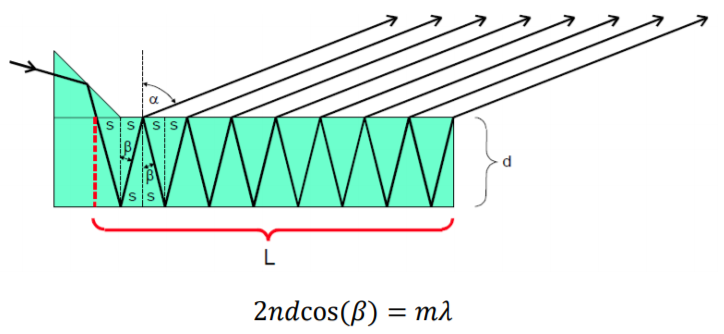
\includegraphics[width=\textwidth]{platte.png}
\caption{Strahlengang in der Lummer-Gehrcke-Platte \cite[2]{anleitung}.}
\label{fig:platte}
\end{figure}

Die LGP zerlegt auftreffendes Licht in einzelne Spektrallinien. Dazu wird die Interferenz an planparallelen Platten
genutzt, um ein hohes Auflösungsvermögen zu erzielen. Das Licht trifft dabei auf ein Prisma und wird auf die planparallele
Platte abgebildet.

Innerhalb der Platte wird das Licht immer wieder reflektiert, wobei bei jeder Reflexion ein kleiner Teil der Strahlen
aus der Platte austritt. Die ausgetretenen Strahlenbündel können konstruktiv miteinander interferieren, solange die Bedingung
dafür gegeben ist.

Bei monochromatischem Licht beträgt der Gangunterschied der Interferenzstreifen genau die Wellenlänge $\lambda$. Wird
jedoch ein Magnetfeld eingeschaltet, so verschieben sich die Wellenlängen um $\delta \lambda$ und die Linien um
$\delta s$.

Damit sich unterschiedliche Ordungen nicht überlagern, dürfen sich die Wellenlängen maximal um

\begin{equation}
  \Delta\lambda_{D} = \frac{\lambda^2}{2d} \sqrt{\frac{1}{n^2-1}}
\end{equation}

unterscheiden. Dabei ist $d$ die Dicke der Platte und $n$ der Brechungsindex.

Die Auflösung der LGP ergibt sich aus

\begin{equation}
  A = \frac{\lambda}{\Delta\lambda} = \frac{L}{\lambda} \left(n^2-1\right) .
\end{equation}

Dabei ist $L$ die Länge der Platte.

Die Aufspaltung der Wellenlänge $\delta \lambda$ errechnet sich aus der Verschiebung der Linien $\delta s$ und der
Differenz $\Delta s$ zwischen dem entsprechenden unaufgespalteten Maximum und dem Maximum der nächsten niedrigeren Ordnung.

\begin{equation}
	\delta \lambda = \frac{1}{2} \frac{\delta s}{\Delta s} \Delta\lambda_{D}
\end{equation}

Damit kann die Aufspaltung der Energie berechnet werden:

\begin{equation}
	E_{auf} = \frac{h c}{\lambda^2} \cdot (2 \delta \lambda) .
\end{equation}
